\section{Experiments}
\label{sec:experiments}

We validate \polar in two settings: online RL rollout and offline SFT data generation.
The experiments test whether unchanged harnesses can produce trainable traces for both reward-driven and supervised training.

\subsection{SWE-Gym GRPO on Coding Harnesses}

\begin{figure}[t]
\centering
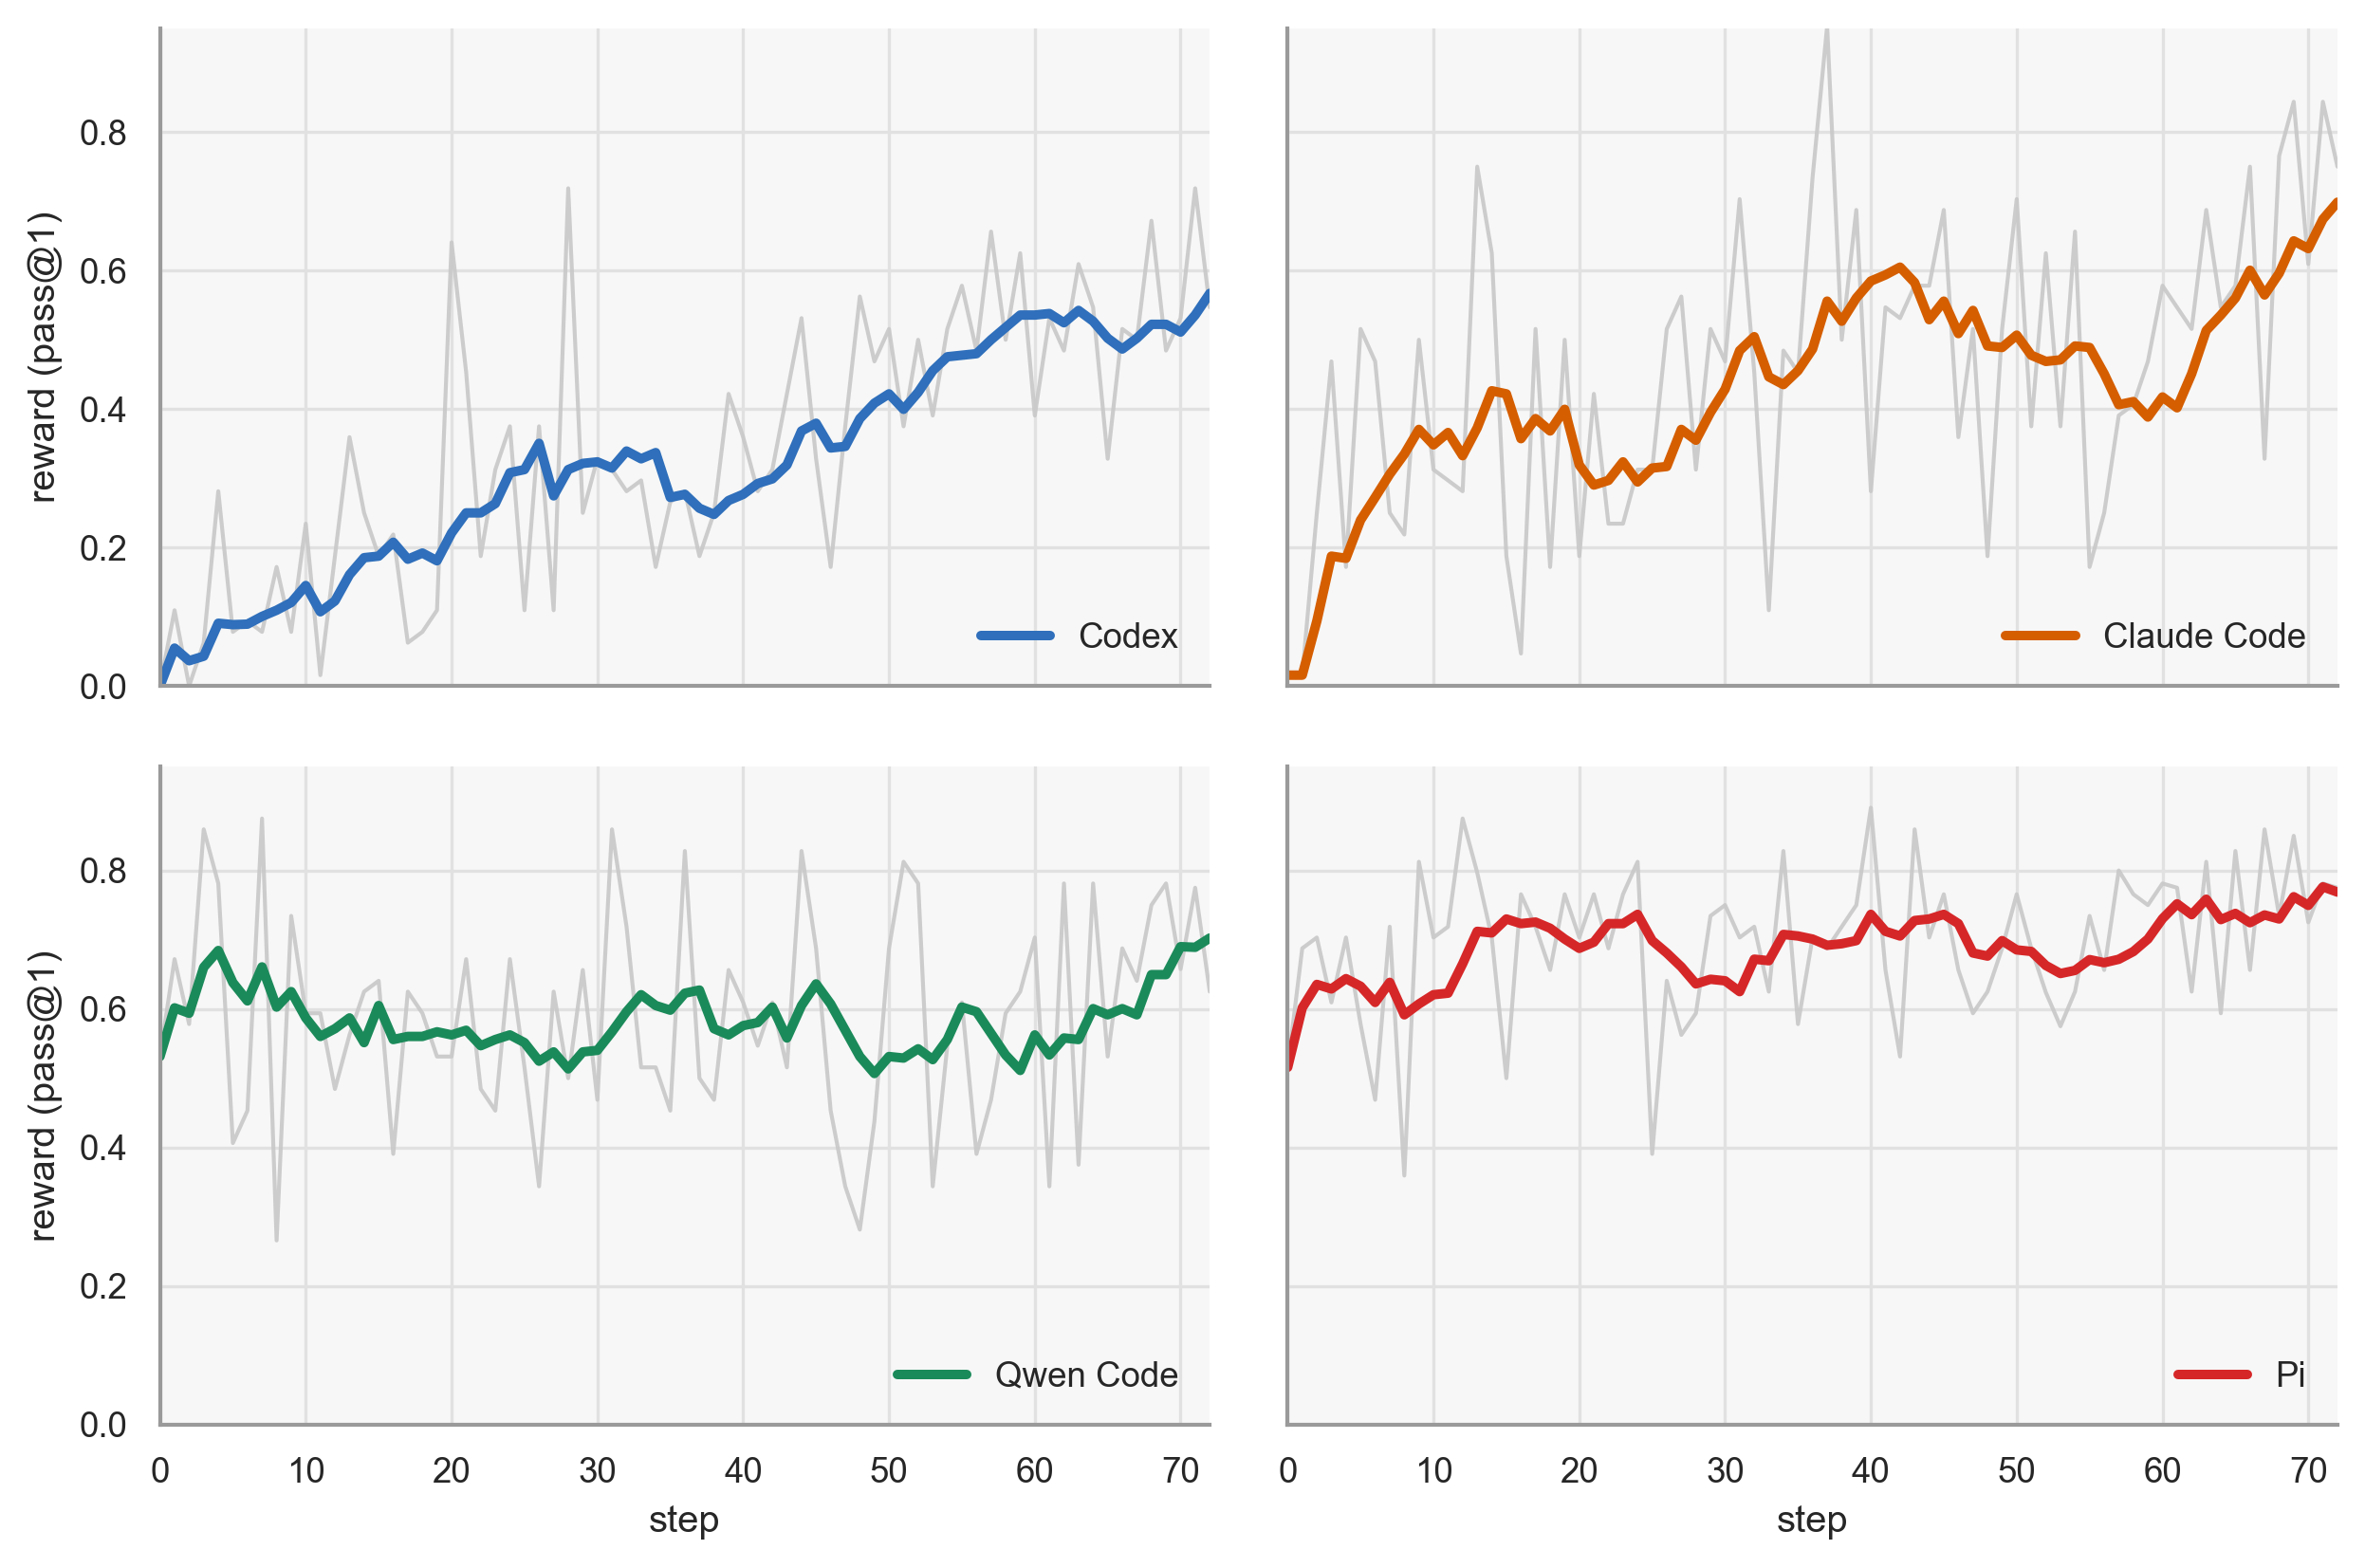
\includegraphics[width=\textwidth]{assets/swegym_grpo_training_curves.png}
\caption{\textbf{SWE-Gym GRPO training curves.} Each panel shows the per-step outcome reward, equivalent to rollout pass@1, for one of four evaluated coding harnesses. RL improves reward across harnesses, with the clear gains on execution paths involving complex prompting, orchestration, or unfamiliar tool schemas.}
\label{fig:swegym_grpo_training_curves}
\end{figure}

We run standard GRPO over four representative coding harnesses with \polar. Starting from the same Qwen3.5-4B base checkpoint, we run standard GRPO training on the \texttt{SkyRL-v0-293-data} SWE-Gym dataset,\footnote{\url{https://huggingface.co/datasets/NovaSky-AI/SkyRL-v0-293-data}} with \polar and Slime.
We use the training split for policy optimization and reserve evaluation for SWE-Bench Verified~\citep{swebench2024}.
All experiments use \texttt{prefix\_merging} to convert llm traffics from harnesses into trainable traces. And we use \texttt{swebench\_harness} to score the final edition patch in a fresh runtime. The main training hyperparameters are listed in \cref{tab:swegym_grpo_hparams}.

\cref{fig:swegym_grpo_training_curves} shows the training reward for Codex, Claude Code, Qwen Code, and Pi. The Codex run begins near zero reward and rises steadily over training, with the last ten steps averaging 54.5\% pass@1 reward compared with 9.5\% over the first ten steps. Claude Code also improves substantially, rising from 28.8\% over the first ten steps to 67.0\% over the last ten steps. Qwen Code and Pi start from stronger native-harness priors: Qwen Code is noisier but rises from 61.6\% to 66.0\%, while Pi improves more clearly from 61.6\% to 76.2\% over the same first and last ten-step windows. These curves are consistent with the benchmark result in \cref{tab:swebench_verified_eval}: \polar improves the same 4B base model under all four evaluated harnesses. The largest absolute gain appear in Codex, likely due to unfamiliar tool schemas.


\begin{table}[t]
\centering
\small
\setlength{\tabcolsep}{8pt}
\begin{tabular}{lccc}
\toprule
\textbf{Harness} & \textbf{Base} & \textbf{\polar RL} & \textbf{Gain} \\
\midrule
Codex & 3.8\% & \textbf{26.4\%} & \textbf{22.6 $\uparrow$} \\
Claude Code & 29.8\% & \textbf{34.6\%} & \textbf{4.8 $\uparrow$} \\
Qwen Code & 34.6\% & \textbf{35.2\%} & \textbf{0.6 $\uparrow$} \\
Pi & 34.2\% & \textbf{40.4\%} & \textbf{6.2 $\uparrow$} \\
\bottomrule
\end{tabular}
\caption{\textbf{SWE-Bench Verified evaluation.} All rows start from the same Qwen3.5-4B base model and are trained over listed harnesses. Scores are pass@1 over the full benchmark, running on corresponding harnesses.}
\label{tab:swebench_verified_eval}
\end{table}

The evaluation isolates the value of harness-native RL. Under Codex, the 4B base model reaches only 3.8\% pass@1 before training, but the \polar-trained checkpoint reaches 26.4\%, a 22.6 point absolute gain. This large jump is expected: Codex presents an unfamiliar action protocol, context policy, and patch-submission style to a Qwen model that was not originally trained as a Codex-native policy. \polar keeps that harness unchanged and attaches the reward to the actual sampled tokens flowing through the Codex execution path, so GRPO optimizes the behavior the model must use at evaluation time. Under the native Qwen Code harness, the base model is already much stronger at 34.6\%, and \polar still improves it to 35.2\%, a 0.6 point gain. Claude Code also improves from 29.8\% to 34.6\%, adding 4.8 points, and Pi improves from 34.2\% to 40.4\%, adding 6.2 points. These results show that harness-native RL can deliver large adaptation gains for unfamiliar execution paths while still preserving gains when the base checkpoint is already well aligned with the harness.


\paragraph{Trajectory builder ablation.}

We ablate the trajectory builder under identical model, hardware, and topology settings, changing only whether captured completions are emitted as \texttt{per\_request} traces or merged by \texttt{prefix\_merging}.
\cref{fig:builder_gpu_utilization} shows a partial utilization profile.
Over same three training steps, \texttt{prefix\_merging} reduces the trainer stream from 1{,}185 request-level updates to 218 merged-trace updates, cutting wall-clock time from 189.5 to 35.2 minutes (5.39$\times$).
\texttt{prefix\_merging} keeps rollout GPUs active with 87.7\% average rollout utilization, compared with 20.4\% average utilization for \texttt{per\_request} over the same period.


We also tried \texttt{per\_request} with outcome-reward broadcasting to every emitted trace, but observed significant reward hacking. The issue is noisy credit assignment: request-level traces can receive session-level credit without proper session normalization or an advanced process reward model. Those mechanisms are outside the scope of this work, but providing examples and tools for session normalization and PRM-style credit assignment is on our roadmap.



\subsection{Offline Data Generation}
\label{sec:offline-data-gen}

Beyond serving online RL rollouts, \polar can be repurposed as a distributed
\emph{offline} data-generation service: a fixed checkpoint and harness are
fanned out across the cluster, every session is journaled to disk, and the
resulting traces are filtered and post-processed for downstream training.
The same primitives that make \polar useful for RL---per-session container
isolation, automatic retry, and gateway-mediated scheduling.

\paragraph{Case study: SWE-Gym SFT trajectories.}
We used \polar to generate a supervised fine-tuning corpus of agentic
software-engineering trajectories. The setup is intentionally minimal: a single
8$\times$H100 SGLang serve job hosting Qwen3.5-122B-A10B (TP$=$8,
\texttt{max\_model\_len}$=$32{,}768) drives the
\texttt{pi-coding-agent}~v0.67.68 harness against 1{,}638 instances drawn from
seven SWE-Gym repositories. Each task runs in its own Apptainer SIF built from
the SWE-Gym reference image with Node.js~22 and the harness layered on top, so
the agent's tool calls (\texttt{bash}, \texttt{read}, \texttt{edit},
\texttt{write}) execute against a fresh checkout of the target commit. Submission
uses \texttt{max\_concurrent}=5--8, \texttt{max\_retries}=1, and a per-task
timeout of 3{,}600 seconds; trajectories that finished with
\texttt{empty\_generation} are retried once and the rest accepted as-is.

A trajectory is accepted into the SFT corpus if and only if the SWE-Bench
evaluation harness reports the agent's final patch as resolving every
\texttt{FAIL\_TO\_PASS} test while leaving every \texttt{PASS\_TO\_PASS} test
green. With this single-bit filter, \polar produced \textbf{504 accepted
trajectories from 1{,}638 attempts} (30.8\% acceptance), at a cost of roughly
64 GPU-hours on the interactive partition. Per-repository acceptance varies
substantially with task difficulty (Table~\ref{tab:swegym-pi-rates}): bug-fix
heavy repositories like \texttt{getmoto/moto} accept at over 50\%, while
data-frame and dataflow workloads with longer test suites accept below 20\%.

\begin{table}[t]
\centering\small
\begin{tabular}{lrrr}
\toprule
\textbf{Repo} & \textbf{Attempts} & \textbf{Accepted} & \textbf{Rate} \\
\midrule
\texttt{getmoto/moto}      & 343 & 184 & 53.6\% \\
\texttt{python/mypy}       & 257 & 101 & 39.3\% \\
\texttt{conan-io/conan}    &  71 &  27 & 38.0\% \\
\texttt{pydantic/pydantic} &  81 &  24 & 29.6\% \\
\texttt{iterative/dvc}     & 219 &  45 & 20.5\% \\
\texttt{pandas-dev/pandas} & 477 &  98 & 19.7\% \\
\texttt{dask/dask}         & 141 &  25 & 17.7\% \\
\midrule
\textbf{Total}             & \textbf{1{,}638} & \textbf{504} & \textbf{30.8\%} \\
\bottomrule
\end{tabular}
\caption{Per-repository acceptance rates for SFT data generated by \polar with
Qwen3.5-122B-A10B and the \texttt{pi} harness on SWE-Gym. ``Accepted'' means
the agent's patch passed both \texttt{FAIL\_TO\_PASS} and \texttt{PASS\_TO\_PASS}
tests in the SWE-Bench evaluator.}
\label{tab:swegym-pi-rates}
\end{table}

\paragraph{Released format.}
Each accepted row contains the SWE-Gym instance metadata
(\texttt{instance\_id}, \texttt{repo}, \texttt{problem\_statement},
\texttt{base\_commit}, \texttt{version}) and the full multi-turn conversation
as a list of OpenAI-style messages with \texttt{role}, \texttt{content},
\texttt{tool\_calls}, and \texttt{tool\_call\_id} fields, terminated by the
assistant turn that produced the accepted patch. Trajectories are long: an
average of 104 messages per session and 51 assistant turns, with a long tail
above 200 turns. The corpus is released as a HuggingFace dataset under an
Apache-2.0 license, with a 90/10 train/test split stratified by repository so
that every repo is represented in both splits.\footnote{Available at
\url{https://huggingface.co/datasets/nvidia/polar-swegym-pi-qwen35-122b-a10b-trajectories}.}

We deliberately kept the filter narrow---a single binary verifier from the
existing SWE-Bench harness---to keep the case study reproducible. The same
\polar deployment can be re-used for richer offline pipelines without changing
the runtime: rejection sampling falls out of running multiple completions per
prompt and keeping only those that pass the verifier; verifier-training data
falls out of retaining the rejected trajectories alongside the accepted ones;
preference data falls out of pairing accepted and rejected traces from the
same prompt. Scaling the present run to the full 2{,}438-instance SWE-Gym set,
swapping in stronger teachers, or adding additional harnesses (e.g.\
\texttt{codex} or \texttt{claude\_code}) requires no changes to the
orchestration code---only additional submitter shards and the corresponding
checkpoint.
